\documentclass{article}

\usepackage{graphicx}
\usepackage{fancyhdr}
\usepackage[sorting=none]{biblatex}
\usepackage[margin=1in]{geometry}
\usepackage{listings}
\usepackage{float}
\usepackage{hyperref}
\usepackage{xepersian}

\addbibresource{bibliography.bib}
\settextfont[Scale=1.2]{B-NAZANIN.TTF}
\setlatintextfont[Scale=1]{Times New Roman}
\renewcommand{\baselinestretch}{1.5}
\pagestyle{fancy}
\fancyhf{}
\rhead{تکلیف دوم درس ریزپردازنده}
\lhead{\thepage}
\rfoot{علیرضا ابره فروش}
\lfoot{9816603}
\renewcommand{\headrulewidth}{1pt}
\renewcommand{\footrulewidth}{1pt}

%%%%%%%%%%%%%%%%
\setcounter{secnumdepth}{3}
\setcounter{tocdepth}{3}
%%%%%%%%%%%%%%%%
\begin{document}
\begin{titlepage}
\begin{center}

\includegraphics[width=0.4\textwidth]{figures/IUT Logo.png}\\
        
\LARGE
\textbf{دانشگاه صنعتی اصفهان}\\
\textbf{دانشکده مهندسی برق و کامپیوتر}\\
        
\vfill
        
\huge
\textbf{عنوان: تکلیف چهارم درس ریزپردازنده}\\
        
\vfill
        
\LARGE
\textbf{نام و نام خانوادگی: علیرضا ابره فروش}\\
\textbf{شماره دانشجویی: 9816603}\\
\textbf{نیم\,سال تحصیلی: پاییز 1400}\\
\textbf{مدرّس: دکتر عارف کریمی افشار}\\
\end{center}
\end{titlepage}


\tableofcontents
\newpage

\section{سوال اول}
\lr{\lstinputlisting[language={[x86masm]Assembler}, showstringspaces=false, basicstyle=\ttfamily]{sources/1.asm}}
\begin{figure}[H]
    \centering
    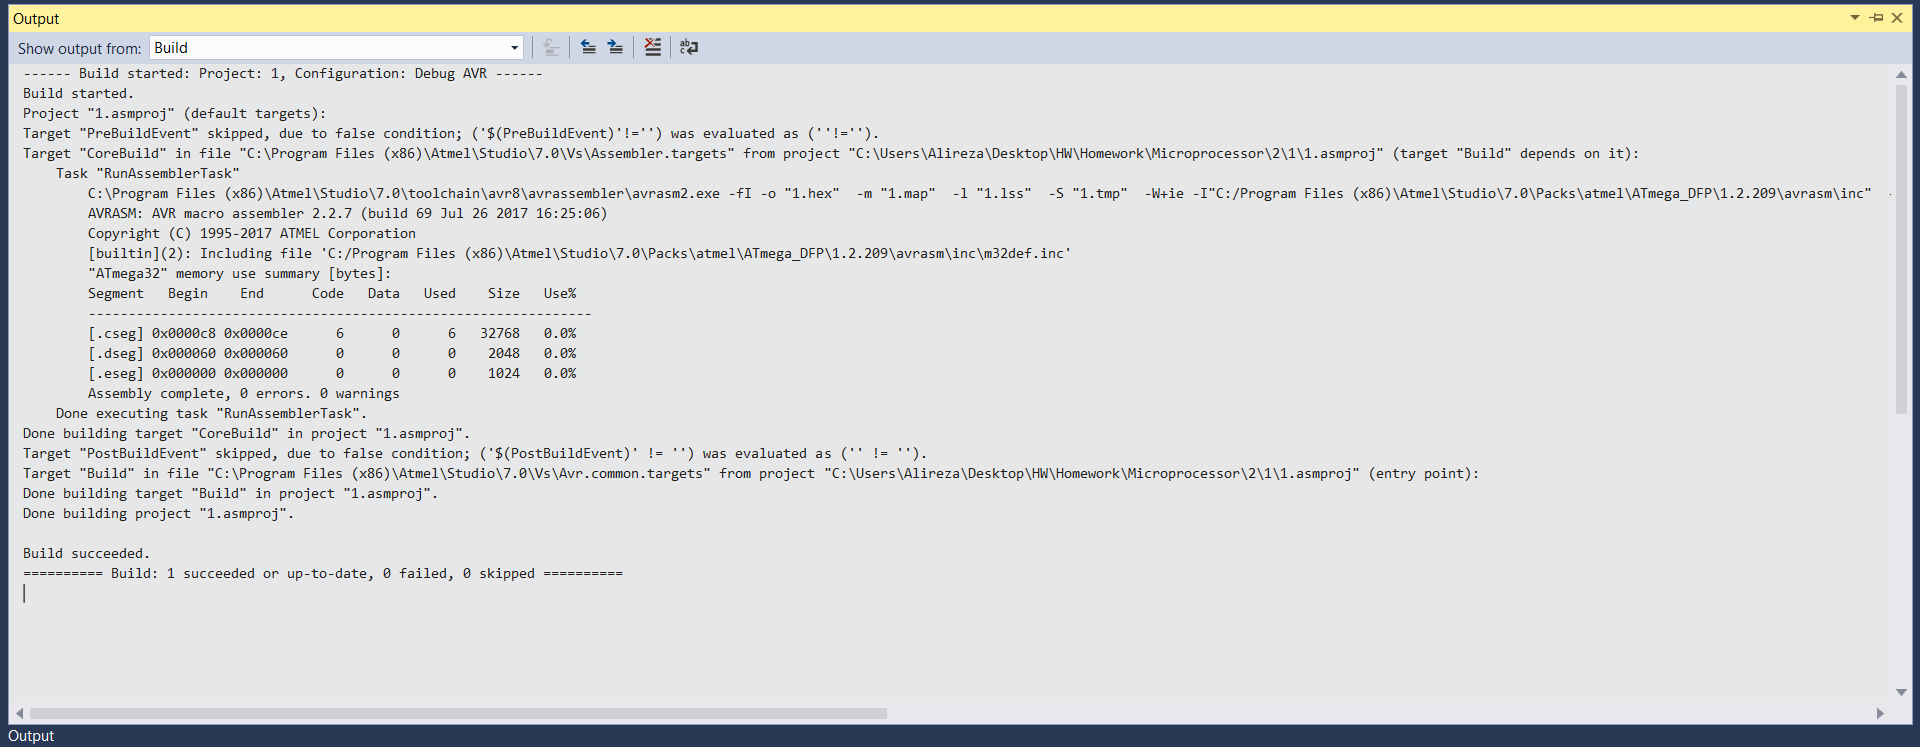
\includegraphics[width=1\textwidth]{figures/1.1.png}
    \caption{خروجی}
    \label{fig:fig1}
\end{figure}
\begin{figure}[H]
    \centering
    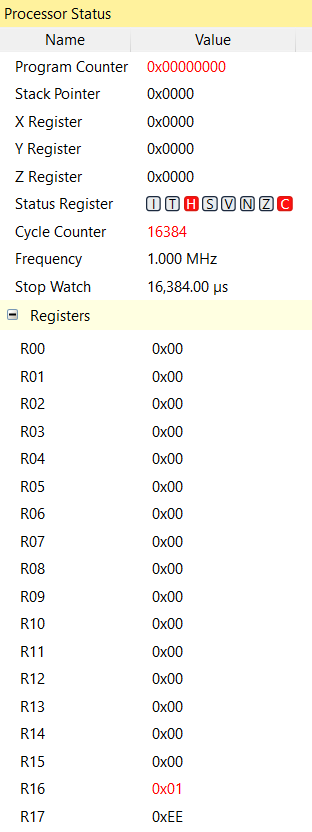
\includegraphics[width=0.25\textwidth]{figures/1.2.png}
    \caption{وضعیت پردازنده}
    \label{fig:fig1}
\end{figure}
در این جمع \lr{Carry}(مجموع دو عدد بدون در نظر گرفتن علامت در مبنای 2 برابر 100000001 است) و \lr{Half Carry}(\lr{Carry} به نیمه دوم منتقل می‌کند) وجود دارد. در نتیجه رجیسترهای وضعیت \lr{H} و \lr{C}، 1 هستند.

\section{سوال دوم}
\lr{\lstinputlisting[language={[x86masm]Assembler}, showstringspaces=false, basicstyle=\ttfamily]{sources/2.asm}}
\begin{figure}[H]
    \centering
    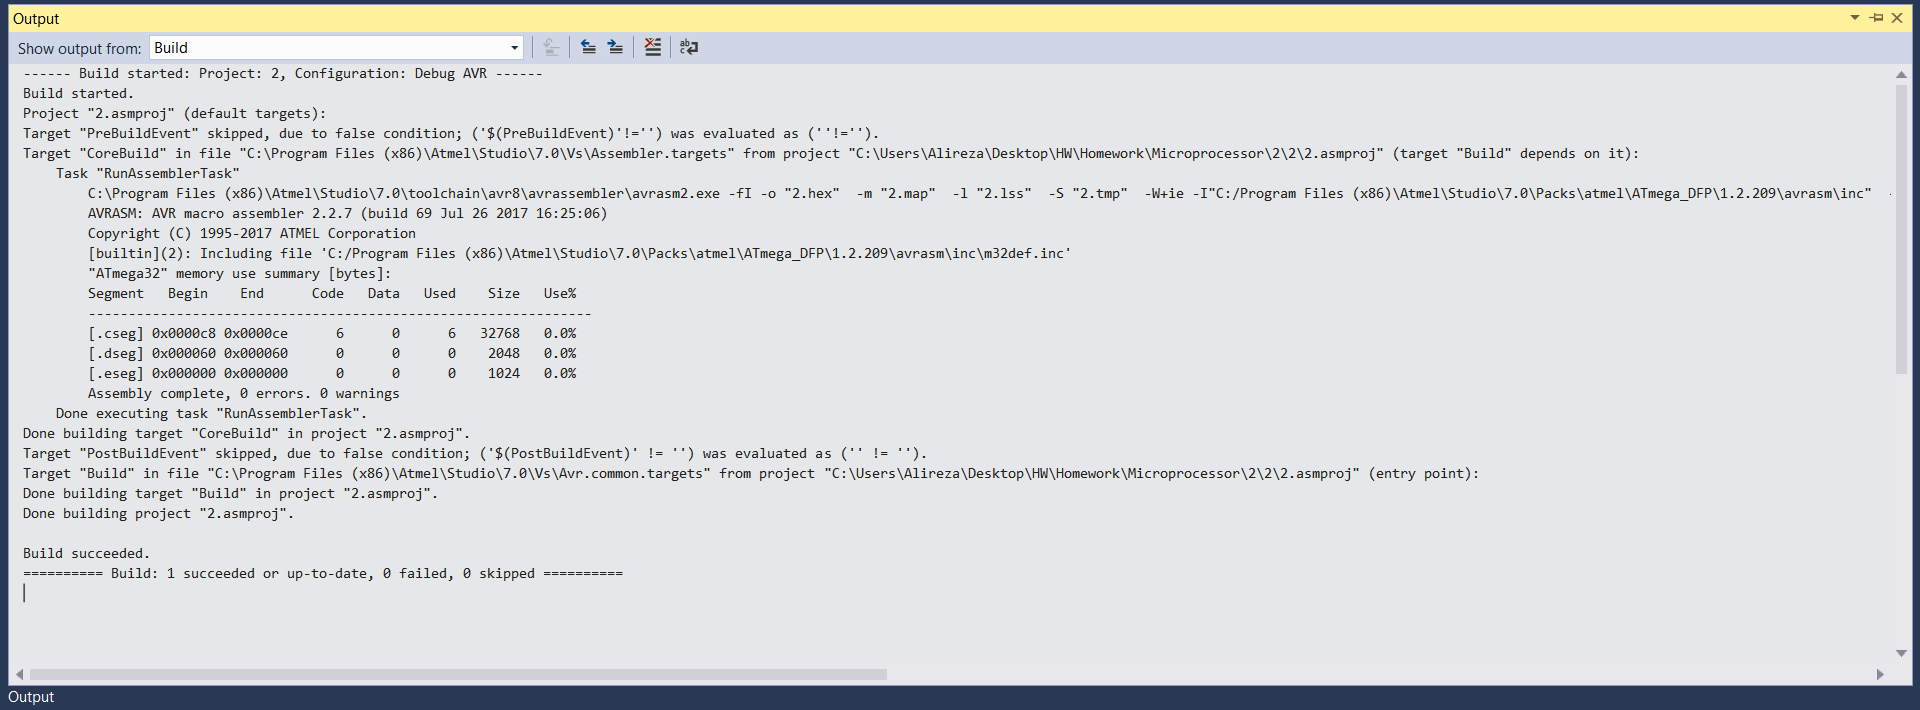
\includegraphics[width=1\textwidth]{figures/2.1.png}
    \caption{خروجی}
    \label{fig:fig1}
\end{figure}
\begin{figure}[H]
    \centering
    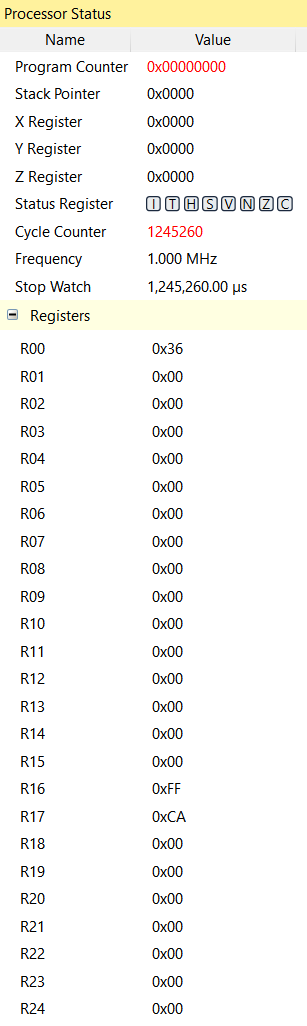
\includegraphics[width=0.25\textwidth]{figures/2.2.png}
    \caption{وضعیت پردازنده}
    \label{fig:fig1}
\end{figure}
ضرب علامتدار انجام گرفته است و نتیجه به درستی در \lr{R0} ریخته شده است.

\section{سوال سوم}
\lr{\lstinputlisting[language={[x86masm]Assembler}, showstringspaces=false, basicstyle=\ttfamily]{sources/3.asm}}
\begin{figure}[H]
    \centering
    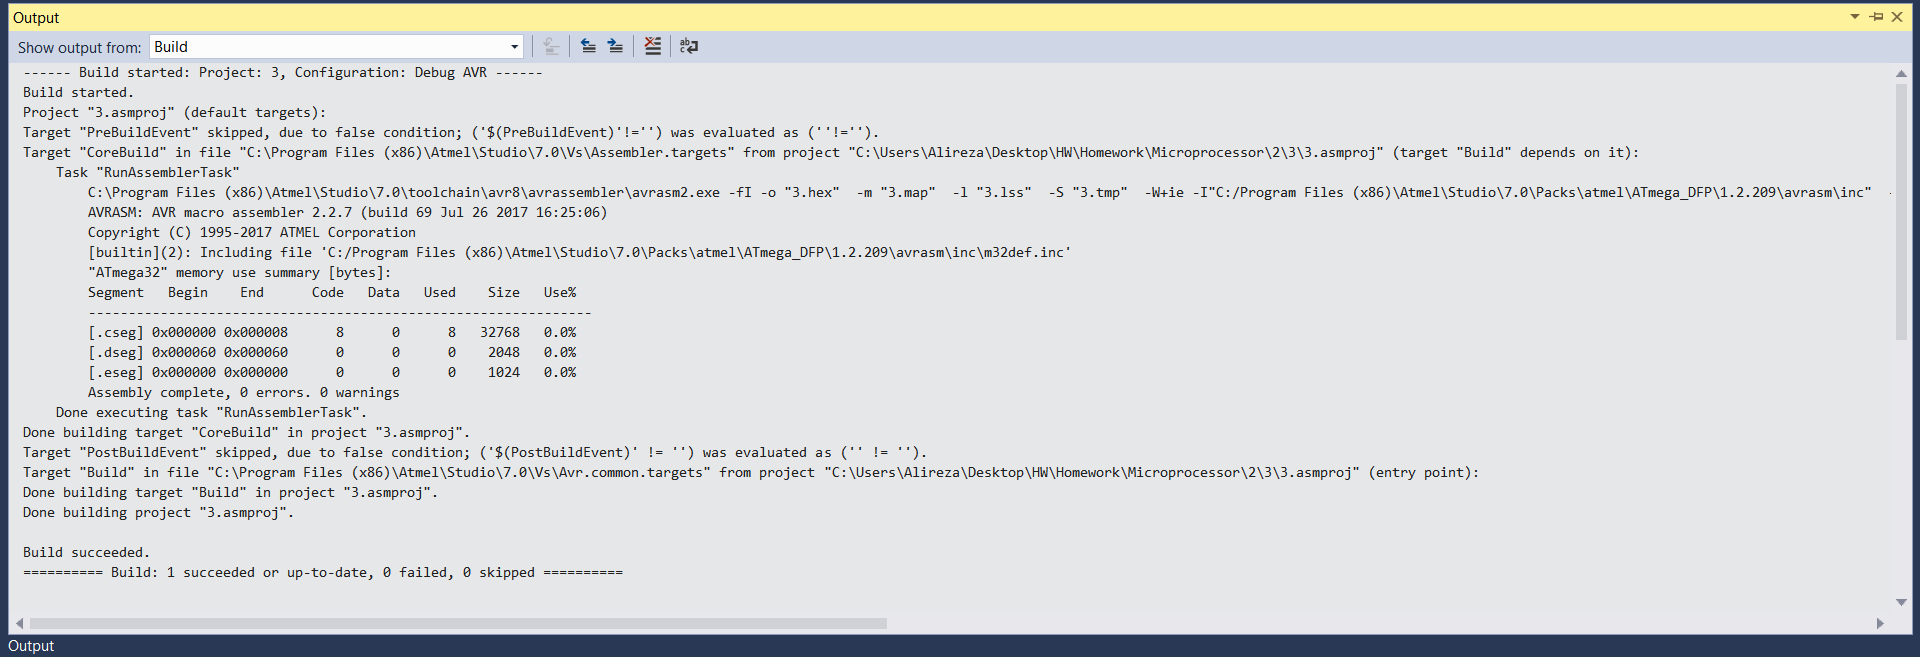
\includegraphics[width=1\textwidth]{figures/3.1.png}
    \caption{خروجی}
    \label{fig:fig1}
\end{figure}
\begin{figure}[H]
    \centering
    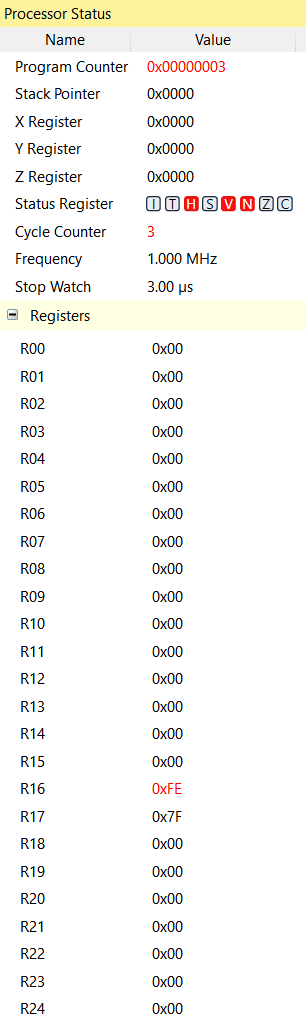
\includegraphics[width=0.25\textwidth]{figures/3.2.png}
    \caption{وضعیت پردازنده}
    \label{fig:fig1}
\end{figure}
هنگامی که 127 و 127 را در مبنای 2 با استفاده از رجیسترهای 8 بیتی جمع می‌کنیم نتیجه 11111110 در مبنای 2 می‌شود که مکمل-2ی عدد 2- است. حاصل جمع منفیِ دو عملوند مثبت(یا بالعکس) نشان‌دهنده‌ی سرریز(\lr{overflow}) است و رجیسترِ \lr{V} را 1 می‌کند.

\section{سوال چهارم}
\lr{\lstinputlisting[language={[x86masm]Assembler}, showstringspaces=false, basicstyle=\ttfamily]{sources/4.asm}}
\begin{figure}[H]
    \centering
    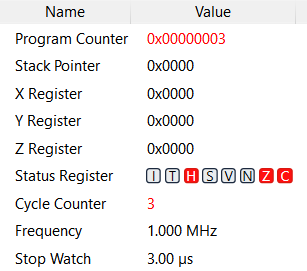
\includegraphics[width=0.5\textwidth]{figures/4.1.png}
    \caption{رجیسترهای وضعیت}
    \label{fig:fig1}
\end{figure}
جمع اعداد در مبنای 16 برابر 100 است. درنتیجه \lr{Carry} داریم. همچنین چون \lr{Carry} به نیمه دوم منتقل می‌شود \lr{Half Carry} داریم. در آخر رجیستر \lr{Z} نشان‌دهنده‌ی این مسئله است که جمع به 00 منتهی شده است.

\section*{منابع}
\renewcommand{\section}[2]{}%
\begin{thebibliography}{99} % assumes less than 100 references
%چنانچه مرجع فارسی نیز داشته باشید باید دستور فوق را فعال کنید و مراجع فارسی خود را بعد از این دستور وارد کنید


\begin{LTRitems}

\resetlatinfont

\bibitem{b1}

\end{LTRitems}

\end{thebibliography}


\end{document}
